\documentclass[a4paper,fontset=none]{ctexart}

\usepackage{anyfontsize}
\usepackage{amsmath,amssymb,mathrsfs,wasysym}
\usepackage{autobreak}
\allowdisplaybreaks
\usepackage[T1]{fontenc}
\usepackage{textcomp}
\usepackage{amsthm}
\usepackage[libertine,vvarbb]{newtxmath}
\usepackage[scr=rsfso,frak=euler,bb=ams]{mathalfa}
\usepackage{bm}
\usepackage{indentfirst}
\setlength{\parindent}{0em}
\usepackage{parskip}
\usepackage{geometry}
\geometry{top=3cm,bottom=3cm,left=2cm,right=2cm}
\usepackage{fontspec}
\setmainfont{Libertinus Serif}
\setsansfont{Libertinus Sans}
\setmonofont{JetBrains Mono}
\setCJKmainfont{SimSun}[BoldFont=Noto Sans CJK SC Medium]
\usepackage{tikz}
\usetikzlibrary{arrows.meta}

\begin{document}

\title{\textbf{天体物理导论作业}}
\author{1900011604\ \ 张植竣\ \ 北京大学}
\date{2021年6月4日}
\maketitle

\section*{第十章}

\begin{itemize}

\item[1.]
观测到的时间差$\delta T$是第三个气壳穿过前两个气壳的时间差$\dfrac{R_\mathrm{e}}{v_3}$减去穿过时辐射从前两个气壳中发射的时间差$\dfrac{R_\mathrm{e}}{c}$，即：
\begin{align*}
    \delta T
    &= \frac{R_\mathrm{e}}{v_3} - \frac{R_\mathrm{e}}{c} \\
    &= \frac{R_\mathrm{e}}{c}\left(1 - \frac{1}{\gamma_3^2}\right)^{-\tfrac{1}{2}} - \frac{R_\mathrm{e}}{c} \\
    &\approx \frac{R_\mathrm{e}}{c}\left(1 + \frac{1}{2\gamma_3^2}\right) - \frac{R_\mathrm{e}}{c} \\
    &= \frac{R_\mathrm{e}}{2c\gamma_3^2} \\
    &\approx \frac{R_\mathrm{e}}{c\gamma^2}
\end{align*}
故估计$\delta T\approx\dfrac{R_\mathrm{e}}{c\gamma^2}$。

\end{itemize}

\section*{第十一章}

\begin{minipage}{0.6\linewidth}

    \begin{itemize}

    \item[1.]
    如右图：
    \[
    x = r\cos\theta,\quad
    y = r\sin\theta
    \]
    \[
    t = \frac{r}{v}
    \]
    \[
    t_{\mathrm{obs}} = t - \frac{x}{c} = \frac{r}{v} - \frac{r\cos\theta}{c} = \frac{r}{v}(1-\beta\cos\theta)
    \]
    \[
    v_{\mathrm{obs}} = \frac{y}{t_{\mathrm{obs}}} = \frac{v\sin\theta}{1-\beta\cos\theta} = c\frac{v\sin\theta}{c-v\cos\theta}
    \]

    \end{itemize}

\end{minipage}
\begin{minipage}{0.36\linewidth}
    \begin{center}
        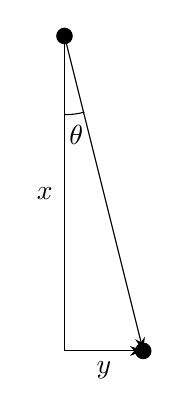
\begin{tikzpicture}[>=Stealth]
            \draw (0,0) -- (0,-4);
            \draw [->] (0,-4) -- (1,-4);
            \draw [->] (0,0) -- (1,-4);
            \fill (0,0) circle [radius=3pt];
            \fill (1,-4) circle [radius=3pt];
            \draw (0,-1) arc [start angle=270,radius=1,delta angle=14.5];
            \draw (0.15,-1.25) node {$\theta$};
            \draw (-0.25,-2) node {$x$};
            \draw (0.5,-4.25) node {$y$};
        \end{tikzpicture}
    \end{center}
\end{minipage}

\section*{第十二章}

\begin{itemize}

\item[1.]

作坐标变换：
\[
x_1 = rR\sin\theta\cos\phi,\quad x_2 = rR\sin\theta\sin\phi,\quad x_3 = rR\cos\theta,\quad x_4 = R\sqrt{1-r^2}
\]
这个变换保证了限制条件$x_1^2+x_2^2+x_3^2+x_4^2=R^2$。相应的坐标微元为：
\begin{align*}
& \mathrm{d}x_1 = -rR\sin\theta\sin\phi\mathrm{d}\phi + rR\cos\theta\cos\phi\mathrm{d}\theta + R\sin\theta\cos\phi\mathrm{d}r \\
& \mathrm{d}x_2 = rR\sin\theta\cos\phi\mathrm{d}\phi + rR\cos\theta\sin\phi\mathrm{d}\theta + R\sin\theta\sin\phi\mathrm{d}r \\
& \mathrm{d}x_3 = -rR\sin\theta\mathrm{d}\theta + R\cos\theta\mathrm{d}r \\
& \mathrm{d}x_4 = -\frac{rR\mathrm{d}r}{\sqrt{1-r^2}}
\end{align*}
先计算$\mathrm{d}x_1^2 + \mathrm{d}x_2^2 + \mathrm{d}x_3^2$如下：
\begin{align*}
    &\quad \mathrm{d}x_1^2 + \mathrm{d}x_2^2 + \mathrm{d}x_3^2 \\
    &= r^2 R^2\sin^2\theta(\sin^2\phi+\cos^2\phi)\mathrm{d}\phi^2 + r^2 R^2\cos^2\theta(\sin^2\phi+\cos^2\phi)\mathrm{d}\theta^2 +  R^2\sin^2\theta(\sin^2\phi+\cos^2\phi)\mathrm{d}r^2 \\
    &\quad + r^2 R^2\sin^2\theta\mathrm{d}\theta^2 + R^2\cos^2\theta\mathrm{d}r^2 + 2rR^2\sin\theta\cos\theta(\sin^2\phi+\cos^2\phi)\mathrm{d}\theta\mathrm{d}r - 2rR^2\sin\theta\cos\theta\mathrm{d}\theta\mathrm{d}r \\
    &= r^2 R^2\sin^2\theta\mathrm{d}\phi^2 + r^2 R^2\mathrm{d}\theta^2 + R^2\mathrm{d}r^2
\end{align*}
则线元$\mathrm{d}l^2$可以表示为：
\begin{align*}
\mathrm{d}l^2
&= \mathrm{d}x_1^2 + \mathrm{d}x_2^2 + \mathrm{d}x_3^2 + \mathrm{d}x_4^2 \\
&= r^2 R^2\sin^2\theta\mathrm{d}\phi^2 + r^2 R^2\mathrm{d}\theta^2 + R^2\mathrm{d}r^2 + \frac{r^2 R^2\mathrm{d}r^2}{1-r^2} \\
&= r^2 R^2\sin^2\theta\mathrm{d}\phi^2 + r^2 R^2\mathrm{d}\theta^2 + \frac{(1-r^2)R^2\mathrm{d}r^2}{1-r^2} + \frac{r^2 R^2\mathrm{d}r^2}{1-r^2} \\
&= r^2 R^2\sin^2\theta\mathrm{d}\phi^2 + r^2 R^2\mathrm{d}\theta^2 + \frac{R^2\mathrm{d}r^2}{1-r^2} \\
&= R^2\left(\frac{\mathrm{d}r^2}{1-r^2} + r^2\mathrm{d}\theta^2 + r^2\sin^2\theta\mathrm{d}\phi^2\right)
\end{align*}

\item[2.]
由于$n_{\mathrm{n}}:n_{\mathrm{p}}=1:7$，而一个$^{1}\mathrm{H}$含有一个质子，一个$^{4}\mathrm{He}$含有两个质子和两个中子，其数密度分别设为$n_{\mathrm{H}}$和$n_\mathrm{He}$，则：
\[
n_{\mathrm{p}} = n_{\mathrm{H}} + 2n_\mathrm{He},\quad
n_{\mathrm{n}} = 2n_\mathrm{He}
\]
即有：
\[
\frac{2n_\mathrm{He}}{n_{\mathrm{H}} + 2n_\mathrm{He}} = \frac{1}{7}
\]
解得：
\[
\frac{n_{\mathrm{H}}}{n_{\mathrm{He}}} = 12
\]
又因为近似有：$m_{\mathrm{He}}=4m_{\mathrm{H}}$，则质量丰度比为：
\[
\frac{m_{\mathrm{H}}}{m_{\mathrm{He}}} = \frac{12}{4} = 3
\]

\end{itemize}

\end{document}